\documentclass[11pt]{article}
\usepackage[utf8]{inputenc}
\usepackage[czech]{babel}
\usepackage{graphicx}

\title{Krásy počítačové grafiky: Triomino}
\author{Tomáš Maršálek}
\date{8.\,března 2012}

\begin{document}
\maketitle

\section{Zadání}
Vytvořte program, který bude skládat Triomino, vstupem bude počet
dělení a velikost jedné strany kresby.

\section{Implementace}
Program je napsán v jazyce Java SE 6. Fraktál triomino je rekurzivně vykreslen
funkcí, která se zastaví po dosažení zadaného počtu dělení. Výsledkem je
rekurzivně vykreslený obrazec tvaru L.  Funkce, která zobrazuje samotné
triomino, postupně vykresluje všechny čtyři dílky L, každý s příslušnou rotací.
Rotace subtriomin a jednotlivých dílků jsou reprezentovány pomocí rotačních
matic.

Velikost strany triomina je zaokrouhlena na nejbližší vyšší mocninu dvou, aby
nedocházelo k zdvojování hran, které je způsobeno zaokrouhlovací chybou.

Abychom vyplnili celou plochu, do zbylého čtverce vpravo nahoře vykreslíme
dalších $n$ menších triomin, kde $n$ je počet dělení.

\begin{figure}[ht!]
\centering
	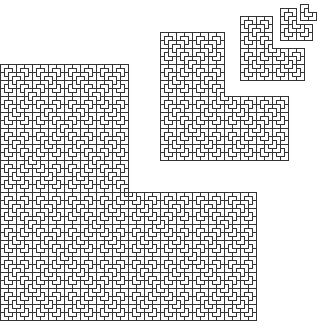
\includegraphics[width=8cm]{triomino_doplneni.png}
	\caption{Doplnění chybějícího horního čtverce}
\end{figure}

\begin{figure}[ht!]
\centering
	
\includegraphics[width=8cm]{triomino5.png}
	\caption{Výsledný fraktál s hloubkou dělení 5}
\end{figure}


\section{Uživatelská příručka}
Program spustíme standardním příkazem pro spuštění java archivů. Parametry
programu jsou počet dělení a velikost jedné strany plátna. Výstupem je triomino
zobrazené v okně.

\begin{verbatim}
java -jar triomino.jar 4 512
\end{verbatim}


\end{document}
